%%%%%%%%%%%%%%%%%%%%%%%%%%%%%%%%%%%%%%%%%%%%%%%%%%%%%%%%%%%%%%%%%%%%%%%%%%
% File: Lecture_1.tex
% Authors: James Kress
% Date: February 1, 2014
% Description: 
%%%%%%%%%%%%%%%%%%%%%%%%%%%%%%%%%%%%%%%%%%%%%%%%%%%%%%%%%%%%%%%%%%%%%%%%%%

%<<<<<<<<<<<<<<<<<<<<<<<<<<<<<<<<<<<<<<<<<<<<<<<<<<<<<<<<<<<<<<<<<<<<<<<<<<<<<%
% Document package information
%>>>>>>>>>>>>>>>>>>>>>>>>>>>>>>>>>>>>>>>>>>>>>>>>>>>>>>>>>>>>>>>>>>>>>>>>>>>>>%
\documentclass[xcolor=dvipsnames]{beamer} 
%%%%%%%%%%%%%%%%%%%%%%%%%%%%%%%%%%%%%%%%%%%%%%%%%%%%%%%%%%%%%%%%%%%%%%%%%%
% File: _TeXdefs.tex
% Author: James Kress
% Date: January 25, 2014
% Description: A tex file containing the \usepackage declarations, and
%			   other document critial style settings.
%%%%%%%%%%%%%%%%%%%%%%%%%%%%%%%%%%%%%%%%%%%%%%%%%%%%%%%%%%%%%%%%%%%%%%%%%%

%-----------Package imports
\usepackage{graphicx}
\usepackage{pgfpages}
\usepackage{tikz}
\usepackage{latexsym}
\usepackage{verbatim}
%//////////END package imports


%----------Style elements
\useoutertheme{infolines} 
\usetheme{Frankfurt} 
\usepackage{../theme/beamercolorthemeoregon}
\setbeamertemplate{sections/subsections in toc}[default]
\setbeamertemplate{footline}
{
\leavevmode%
  \hbox{%
  \begin{beamercolorbox}[wd=.3\paperwidth,ht=2.25ex,dp=.75ex,center]{institute in head/foot}%
    \usebeamerfont{institute in head/foot}\insertshortinstitute
  \end{beamercolorbox}%
    \begin{beamercolorbox}[wd=.4\paperwidth,ht=2.25ex,dp=.75ex,center]{title in head/foot}%
      \usebeamerfont{title in head/foot}\insertshorttitle
    \end{beamercolorbox}%
  \begin{beamercolorbox}[wd=.3\paperwidth,ht=2.25ex,dp=.75ex,center]{date in head/foot}%
    \usebeamerfont{date in head/foot}\insertshortdate\hspace*{3em}
    \insertframenumber{} / \inserttotalframenumber\hspace*{1ex}
  \end{beamercolorbox}}%
  \vskip0pt%
}
%/////////END style elements


%---------Command Declarations
\DeclareGraphicsExtensions{.pdf, .jpeg, .png, .jpg}
\graphicspath{ {../images/} }
\newcommand{\className}{\text{CIS 410/510} \\ \text{Parallel Computing}}
\newcommand{\departmentName}{\textit{Department of Computer and 
									Information Science \\ University of Oregon}}
%/////////END command declarations


%---------Setup pdf properties
\hypersetup{
	pdfusetitle=true,
    bookmarks=true,         	% show bookmarks bar?
    unicode=false,          	% non-Latin characters in Acrobat’s bookmarks
    pdftoolbar=true,        	% show Acrobat’s toolbar?
    pdfmenubar=true,        	% show Acrobat’s menu?
    pdffitwindow=false,     	% window fit to page when opened
    pdfstartview={Fit},   		% fits the width of the page to the window    
    pdfauthor={},     % author
    pdfsubject={Parallel Programming},   	% subject of the document
    pdfcreator={},   			% creator of the document
    pdfproducer={}, 			% producer of the document
    pdfkeywords={University of Oregon, parallel programming}, 
    pdfnewwindow=true,      	% links in new window
    colorlinks=true,       		% false: boxed links; true: colored links
    linkcolor=white,          	% color of internal links
    hidelinks,
    citecolor=green,        	% color of links to bibliography
    filecolor=magenta,      	% color of file links
    urlcolor=cyan,           	% color of external links
    linktoc=page,
    pageanchor = true
}
%//////////END setup pdf properties


%END ALL


%<<<<<<<<<<<<<<<<<<<<<<<<<<<<<<<<<<<<<<<<<<<<<<<<<<<<<<<<<<<<<<<<<<<<<<<<<<<<<%
% END Document package information
%>>>>>>>>>>>>>>>>>>>>>>>>>>>>>>>>>>>>>>>>>>>>>>>>>>>>>>>>>>>>>>>>>>>>>>>>>>>>>%

%=============================================================================%
% Begining: Title Page Material
%=============================================================================%
\begin{document}
	\title[Map Pattern]{Map Pattern}
	\author[]{\className}
	\institute[\className]{\departmentName}
	\date{} 

	\titlegraphic{\centering 
		$\vcenter{\hbox{
\includegraphics[height=.31in,width=2.0in]{oregonLogo}}}$
	}

	\begin{frame}
		\maketitle
	\end{frame}
	
	\begin{frame}{Developer Training}
		\begin{center}
			
\includegraphics[width=0.4\textwidth]{images/OSNAP_logo} 
			
			Map Pattern
			
			Executive PIN Recovery
		\end{center}
	\end{frame}
	
	\begin{frame}{Executive PIN Recovery}
		\begin{columns}
			\begin{column}{0.5\textwidth}
					O-SNAP security policies demand workers use an 8 digit pin, changed daily, to 
					access secured resources. \\~\\
					Executive management has requested a pin recovery tool since they tend to forget 
					the pins. To be compliant with the organizational security policies, no system or 
					person may keep pins in plain text or reversibly encrypted. md5 checksums of the 
					pin have no confidentiality requirements according to O-SNAP security policy.
			\end{column}
			\begin{column}{0.5\textwidth}
				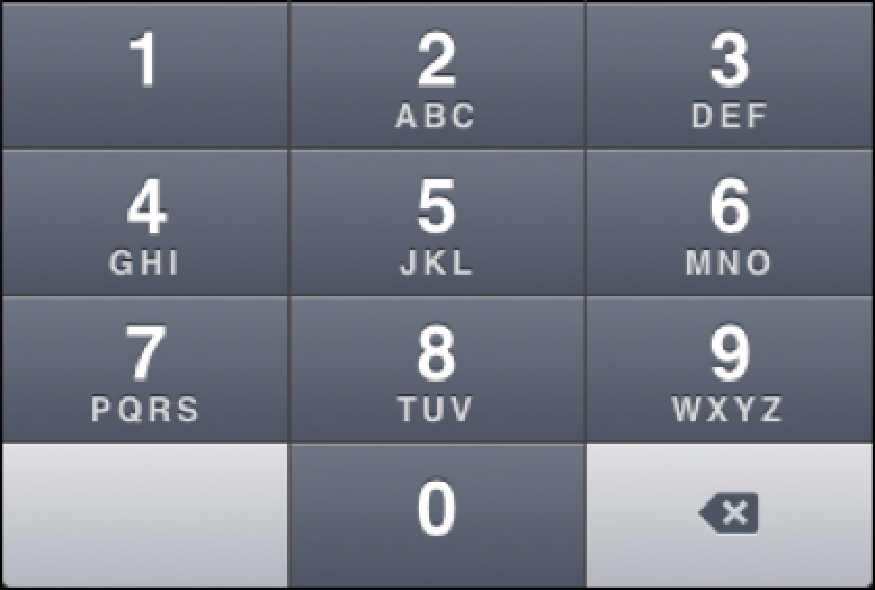
\includegraphics[width=\textwidth]{images/keypad}
			\end{column}
		\end{columns}
	\end{frame}
	
	\begin{frame}{Basic Solution}
		\begin{itemize}
			\item Have the user carry a hashed copy of the pin
			\item Enter the hashed copy to the software
			\item Software hashes all possible pins
			\item Software returns the pin that matches the entered hash
			\item \href{http://ix.cs.uoregon.edu/~dellswor/410}{\url{http://ix.cs.uoregon.edu/~dellswor/410}}
		\end{itemize}
	\end{frame}
	%--- Next Frame ---%
	
  \begin{frame}{Map Pattern}
		\begin{columns}
			\begin{column}{0.5\textwidth}
				\begin{itemize}
					\item N atomic data units
					\item 1-to-1 mapping of work units to compute units
					\item Compute units all apply the same atomic computation
				\end{itemize}
			\end{column}
			\begin{column}{0.5\textwidth}
				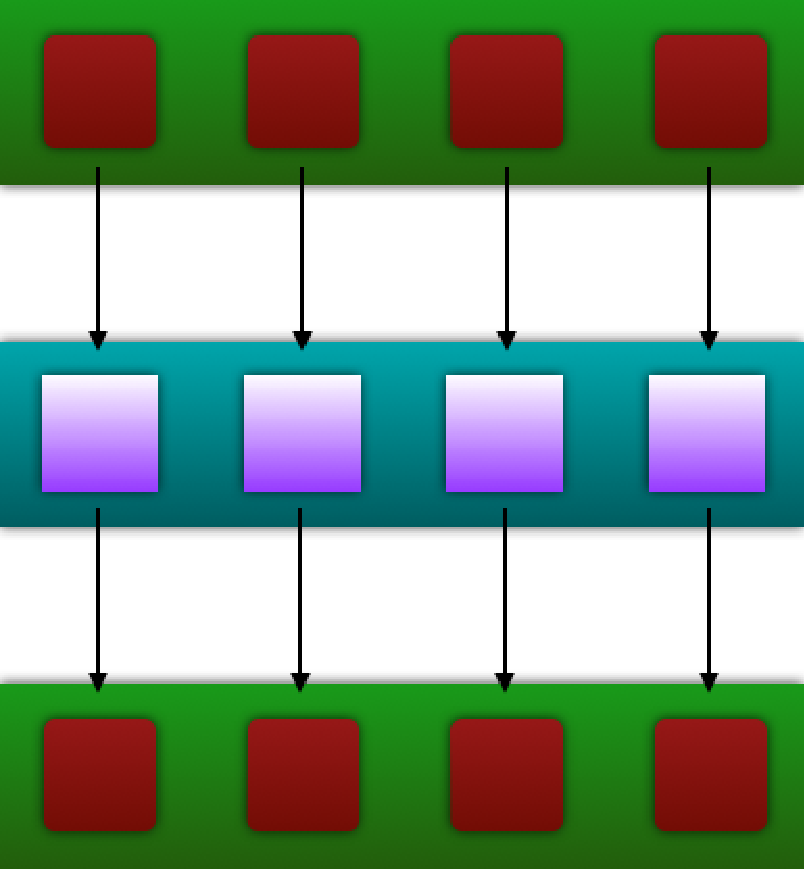
\includegraphics[width=\textwidth]{images/mapPattern}
			\end{column}
		\end{columns}
	\end{frame}
	
	
	\begin{frame}{Multiple Passwords}
		\begin{itemize}
			\item Instead of cracking just one executive pin, crack a set of them
			\item Discussion: How do we parallelize this?
		\end{itemize}
	\end{frame}
	
	\begin{frame}{Multiple Passwords - Example code}
		\begin{itemize}
      \item Example code is stored on Mist
      \item Get into a directory you store source in 
			\item On Mist: run "cp -r /home/users/poliadz/ParallelPasswordCracker ."
		\end{itemize}
	\end{frame}
	
  \begin{frame}{Homework}
	\begin{itemize}
		\item Assignment: Convert an image into ASCII art
		\item Note: You will use this in later labs to display your results
		\item Details: \href{https://github.com/UOregonParallel/CourseMaterials/wiki/ASCII-Art}{\url{https://github.com/UOregonParallel/CourseMaterials/wiki/ASCII-Art}}
	\end{itemize}
  \end{frame}
  
  \begin{frame}{Key Points - Map}
		\begin{itemize}
      \item Concept: apply the same operation to multiple data elements independently
      \item Design: Challenge in map is ensuring operations do the same amount of work
			\item Identifying the correct parallelization is key to performance
		\end{itemize}
	\end{frame}
	
	%--- Next Frame ---%

\end{document}
%END ALL

